\subsection*{Цель}

Отработка навыков использования программы Microsoft Project для оптимизации временных и финансовых показателей проекта.

\subsection*{Задание 1: выравнивание загрузки ресурсов}

В проекте была перегрузка ресурсов:

\begin{enumerate}
    \item системный аналитик --- должен параллельно выполнять задачи <<Анализ и построение структуры базы объектов>> и <<Анализ и проектирование ядра>> c 01.03 по 15.03.
    \item художник-дизайнер --- перегружен задачами <<Разработка дизайна руководства>> и <<Разработка дизайна сайта>> c 02.08 по 05.08.
    \item технический писатель --- накладывались задачи <<Написание руководства пользователя>> и <<Создание справочной системы>> с 13.08 по 21.08.
\end{enumerate}

\begin{figure}[h!]
	\begin{center}
		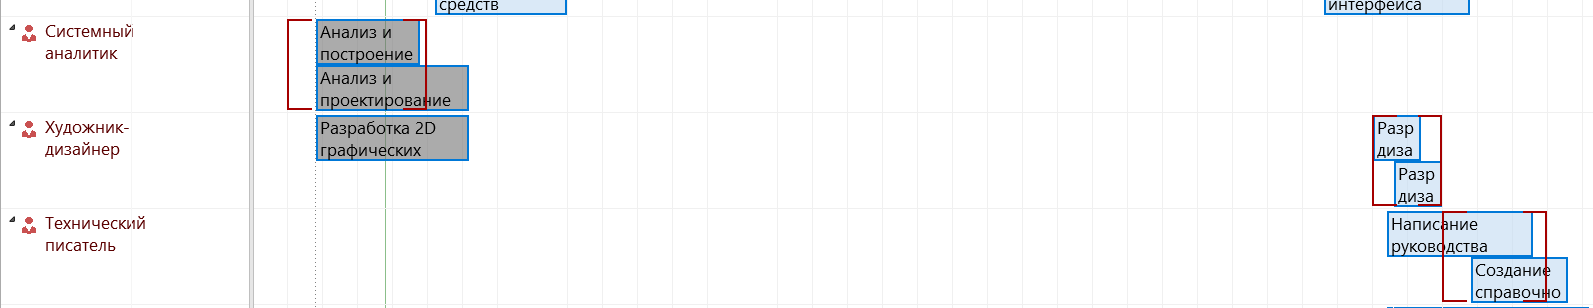
\includegraphics[scale=0.4]{inc/img/p_1.png}
	\end{center}
	\captionsetup{justification=centering}
	\caption{Перегрузка из-за наложения задач}
	\label{fig:u3}
\end{figure}

Автоматическое выравнивание применяется для устранения перегрузки ресурсов путем изменения продолжительности задачи или дробления ее на несколько подзадач.

Было выполнено автоматическое выравнивание ресурсов (Ресурс → Выровнять все) с параметрами выравнивания по умолчанию (вкладка Ресурс → Параметры выравнивания). 

\begin{figure}[h!]
	\begin{center}
		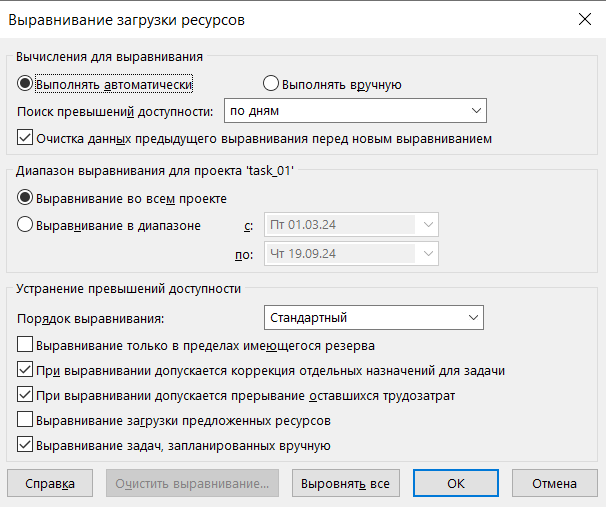
\includegraphics[scale=0.8]{inc/img/p_2.png}
	\end{center}
	\captionsetup{justification=centering}
	\caption{Параметры выравнивания}
	\label{fig:u3}
\end{figure}

Внесенные изменения после выравнивания (Вид → Другие представления → Диаграмма Ганта с выравниванием) приведены на рисунке. Зеленые планки означают исходные параметры до выравнивания, синие (если они есть) означают задержки, добавленные при выравнивании. Выделены
изменившиеся задачи.

\begin{figure}[h!]
	\begin{center}
		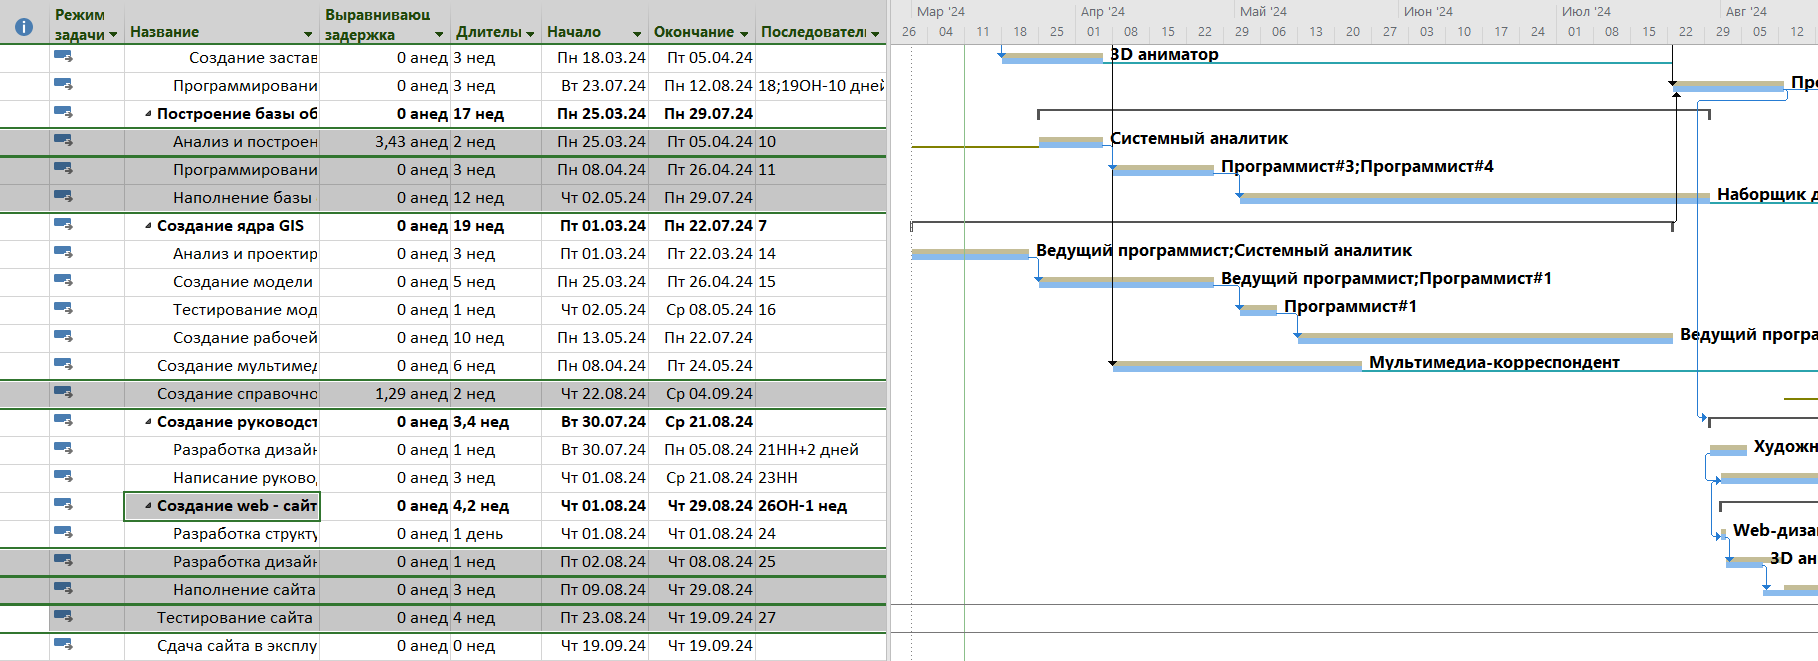
\includegraphics[scale=0.34]{inc/img/p_3.png}
	\end{center}
	\captionsetup{justification=centering}
	\caption{Диаграмма Ганта после выравнивания}
	\label{fig:u3}
\end{figure}

\newpage

Анализ изменений:

\begin{enumerate}
    \item Сместилось вперед время начала выполнения задачи 9 (а за ней 10 и 11 из-за их последовательных связей), чтобы разгрузить ресурс «Системный аналитик», который в это время будет заниматься задачей 13.
    \item Сместилось вперед время начала выполнения задачи 18, чтобы разгрузить ресурс «Технический писатель», который в это время будет заниматься задачей 21 (заканчивать ее).
    \item Увеличилась продолжительность выполнения задачи 24 (а за ней сместилось время начала выполнения задач 25 и 26 из-за их последовательных связей), чтобы ресурс «Художник-дизайнер» мог приступить к своей части работы позже, чтобы успеть сначала закончить задачу 20.
\end{enumerate}

Первые два два изменения обусловлены тем, что данные задачи не находятся на критическом пути, и их выполнения последовательно, а не параллельно, не скажется на времени выполнения проекта.


\textbf{}

\textbf{Результат}: после выравнивания ресурсы более не перегружены.

\vspace{8pt}

\begin{figure}[h!]
	\begin{center}
		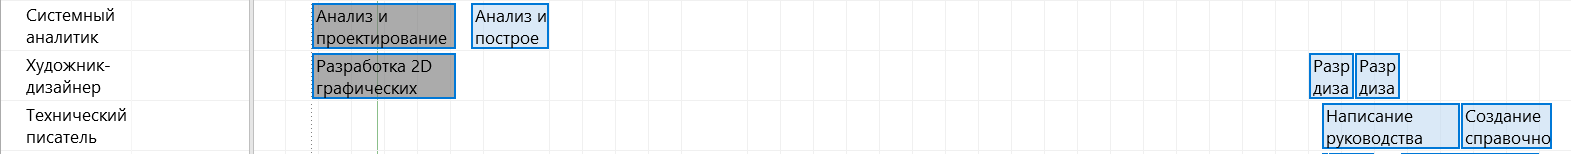
\includegraphics[scale=0.42]{inc/img/p_4.png}
	\end{center}
	\captionsetup{justification=centering}
	\caption{Ресурсы после выравнивания}
	\label{fig:u3}
\end{figure}

\newpage

\subsection*{Задание 2: учёт периодических задач в плане проекта}

В плане проекта отражено проведение еженедельного совещания по
средам с 10 до 11 утра. 

\begin{figure}[h!]
	\begin{center}
		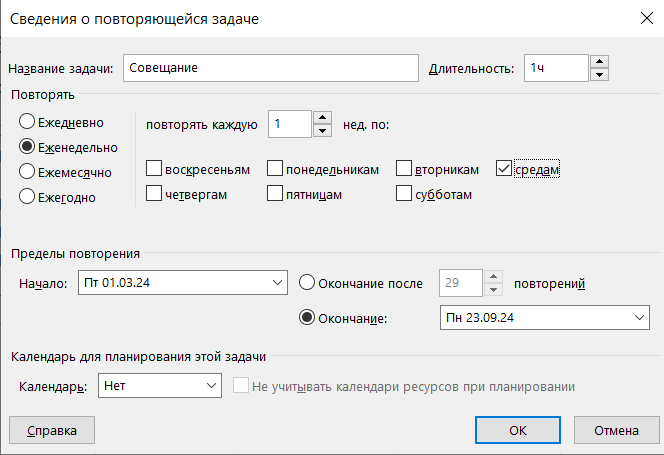
\includegraphics[scale=0.75]{inc/img/p_5.png}
	\end{center}
	\captionsetup{justification=centering}
	\caption{Создание новой задачи}
	\label{fig:u3}
\end{figure}

К участию в совещании привлечены все специалисты, кроме
наборщиков данных и программистов №1-4 (их интересы на совещании представляет ведущий программист). 

\begin{figure}[h!]
	\begin{center}
		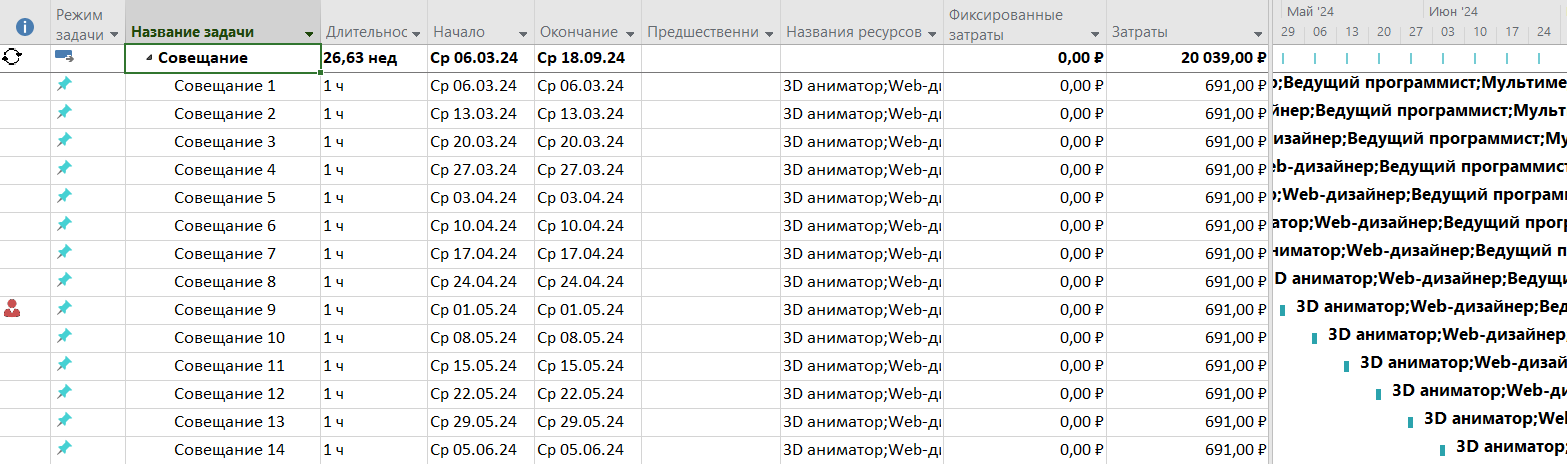
\includegraphics[scale=0.4]{inc/img/p_6.png}
	\end{center}
	\captionsetup{justification=centering}
	\label{fig:u3}
\end{figure}

Возникли перегрузки из-за того, что совещания происходят в рабочее время.

\begin{figure}[h!]
	\begin{center}
		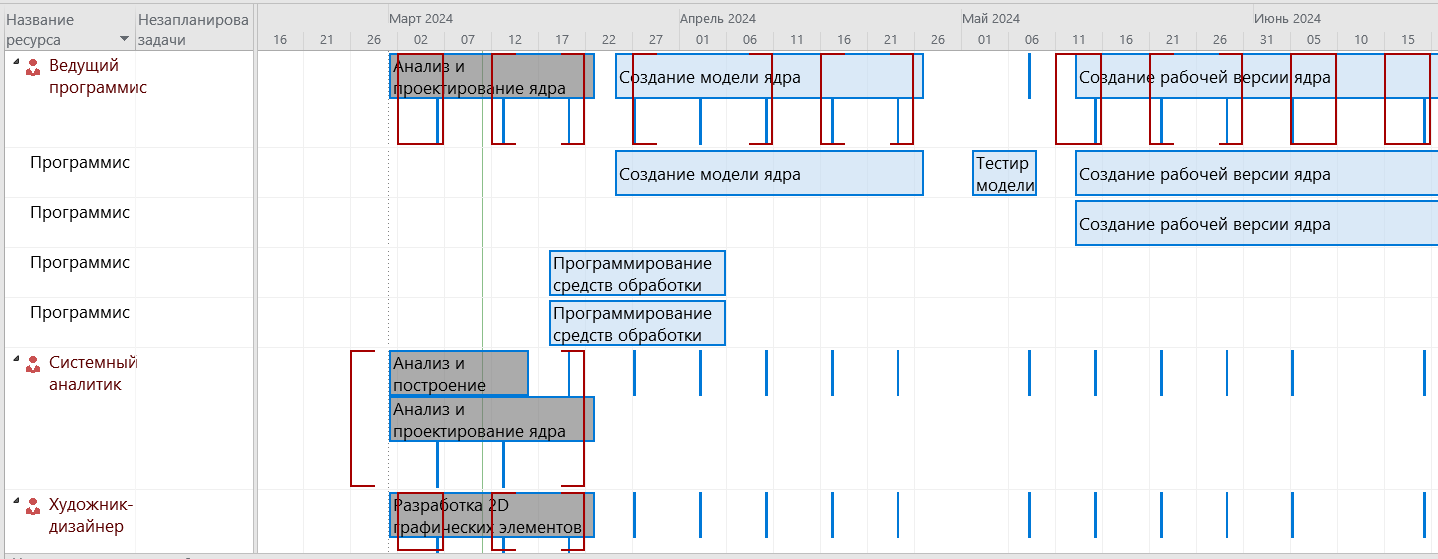
\includegraphics[scale=0.43]{inc/img/p_7.png}
	\end{center}
	\captionsetup{justification=centering}
	\label{fig:u3}
\end{figure}

Устранена перегрузка ресурсов с помощью автоматического
выравнивания. Также удалены совещания 1 мая и 12 июня, так как это праздничные дни.

\begin{figure}[h!]
	\begin{center}
		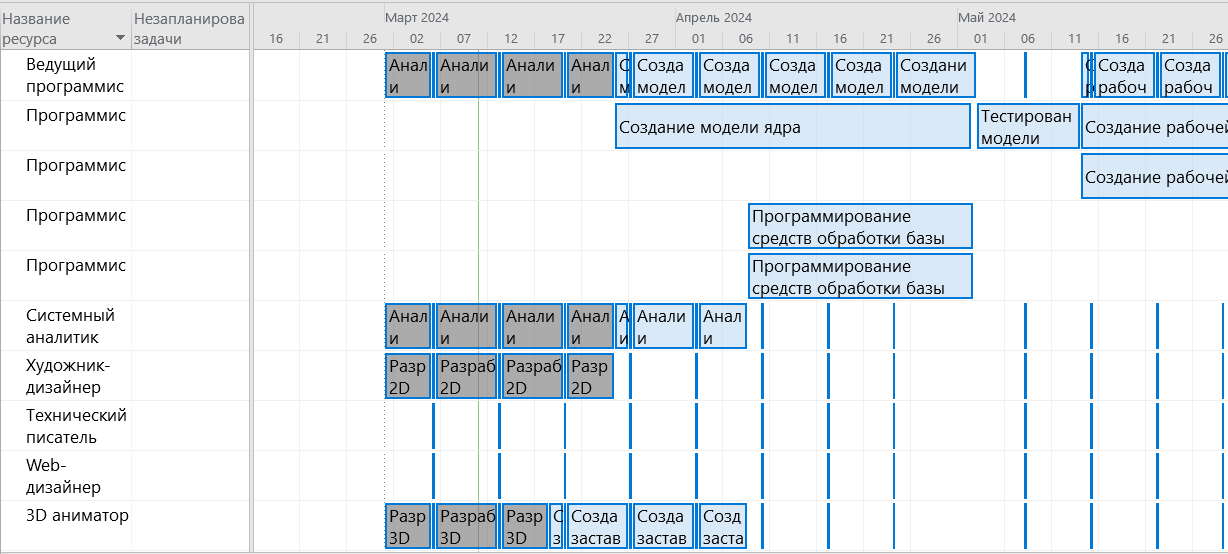
\includegraphics[scale=0.47]{inc/img/p_8.png}
	\end{center}
	\captionsetup{justification=centering}
	\label{fig:u3}
\end{figure}

\begin{figure}[h!]
	\begin{center}
		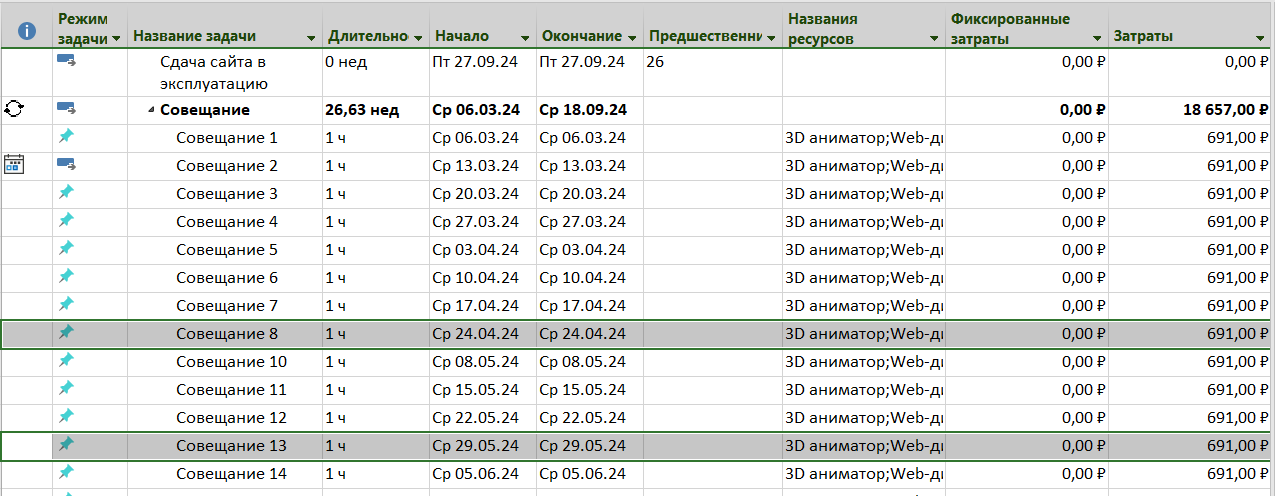
\includegraphics[scale=0.45]{inc/img/p_9.png}
	\end{center}
	\captionsetup{justification=centering}
	\label{fig:u3}
\end{figure}

В результате перегрузки ресурсов были устранены.

После введения совещаний и выравнивания были добавлены перерывы
в выполнении задач, поэтому срок выполнения проекта увеличился до 28.65 недель, а затраты – до 66835р, что превышает выделенный срок в 6 месяцев и бюджет в 50000р. 

\begin{figure}[h!]
	\begin{center}
		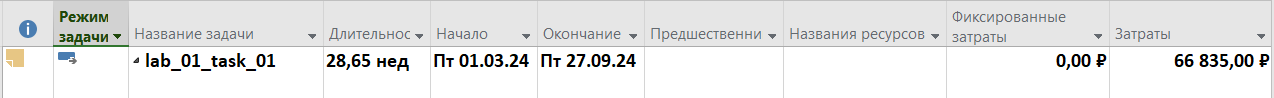
\includegraphics[scale=0.45]{inc/img/p_10.png}
	\end{center}
	\captionsetup{justification=centering}
	\label{fig:u3}
\end{figure}

Поскольку превышены сроки и бюджет, необходимо провести
оптимизацию временных и финансовых параметров проекта.

Для оптимизации финансовых параметров необходимо учесть, что во время совещаний сотрудники, участвующие в нем, не заняты своей основной работой, поэтому можно создать отдельный план затрат B, в котором не будет затрат на использование, для каждого из этих ресурсов на время совещаний. Пример такого плана для ресурса «Web-дизайнер» приведен на рисунке.

\begin{figure}[h!]
	\begin{center}
		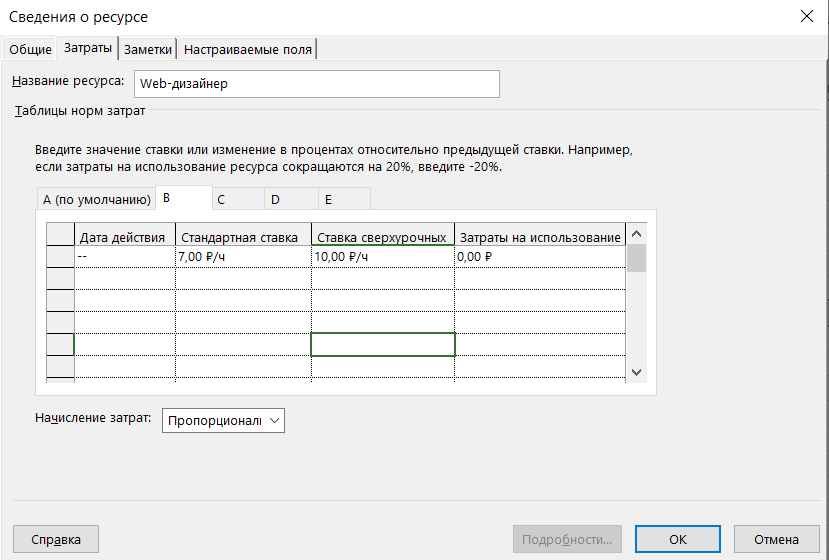
\includegraphics[scale=0.6]{inc/img/p_11.png}
	\end{center}
	\captionsetup{justification=centering}
	\label{fig:u3}
\end{figure}

Этот план затрат указан в столбце «Таблица норм затрат» для каждого совещания:

\begin{figure}[h!]
	\begin{center}
		
\includegraphics[scale=0.6]{inc/img/p_12.png}
	\end{center}
	\captionsetup{justification=centering}
	\label{fig:u3}
\end{figure}

\newpage

Таким образом, затраты уменьшились до 49825р, и теперь находятся в рамках
выделенного бюджета:

\begin{figure}[h!]
	\begin{center}
		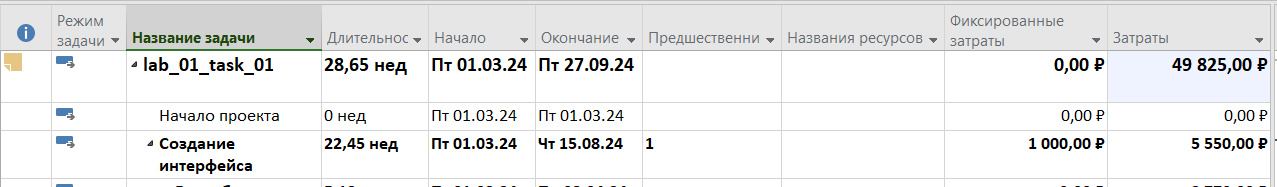
\includegraphics[scale=0.48]{inc/img/p_13.png}
	\end{center}
	\captionsetup{justification=centering}
	\label{fig:u3}
\end{figure}

\clearpage

\subsection*{Задание 3: оптимизация критического пути}

Перед началом оптимизации дата окончания проекта – 27.09.2024.

Критический путь (Вид → Фильтр → Критические задачи):

\begin{figure}[h!]
	\begin{center}
		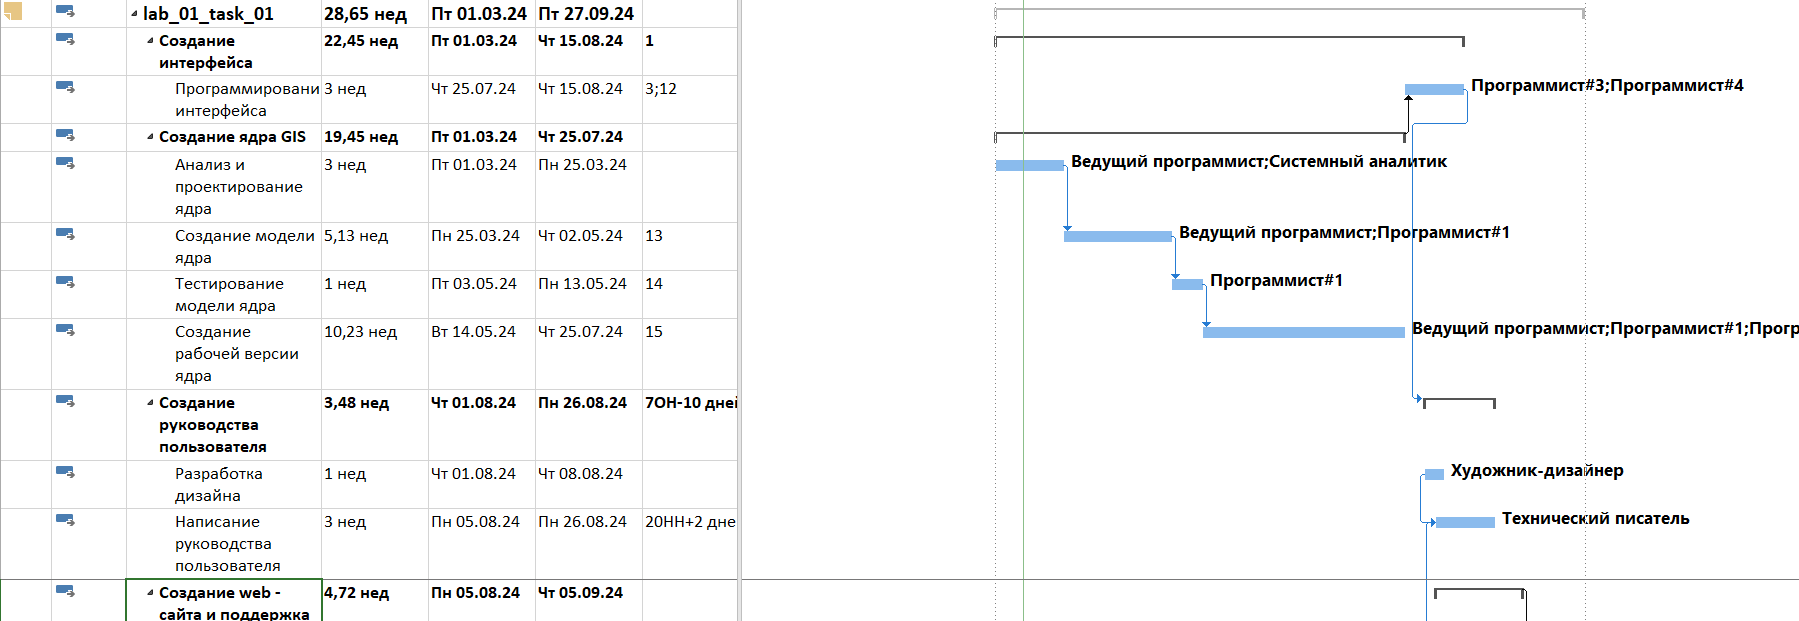
\includegraphics[scale=0.35]{inc/img/p_14.png}
	\end{center}
	\captionsetup{justification=centering}
	\label{fig:u3}
\end{figure}

Наибольшее влияние на срок реализации проекта оказывает фаза 12 (в особенности – задачи 16 и 14). Она наиболее продолжительная, и только после нее начинают выполняться остальные задачи критического пути. Также
сравнительно длинной является задача 25.
Во всех этих задачах используются программисты.
На вкладе «Визуальный оптимизатор ресурсов» видно, что программисты используются нерационально: пока одни заняты в задаче (например, первый и второй занимаются задачей создания рабочей версии ядра), остальные (3 и 4)
свободны, и наоборот.

\begin{figure}[h!]
	\begin{center}
		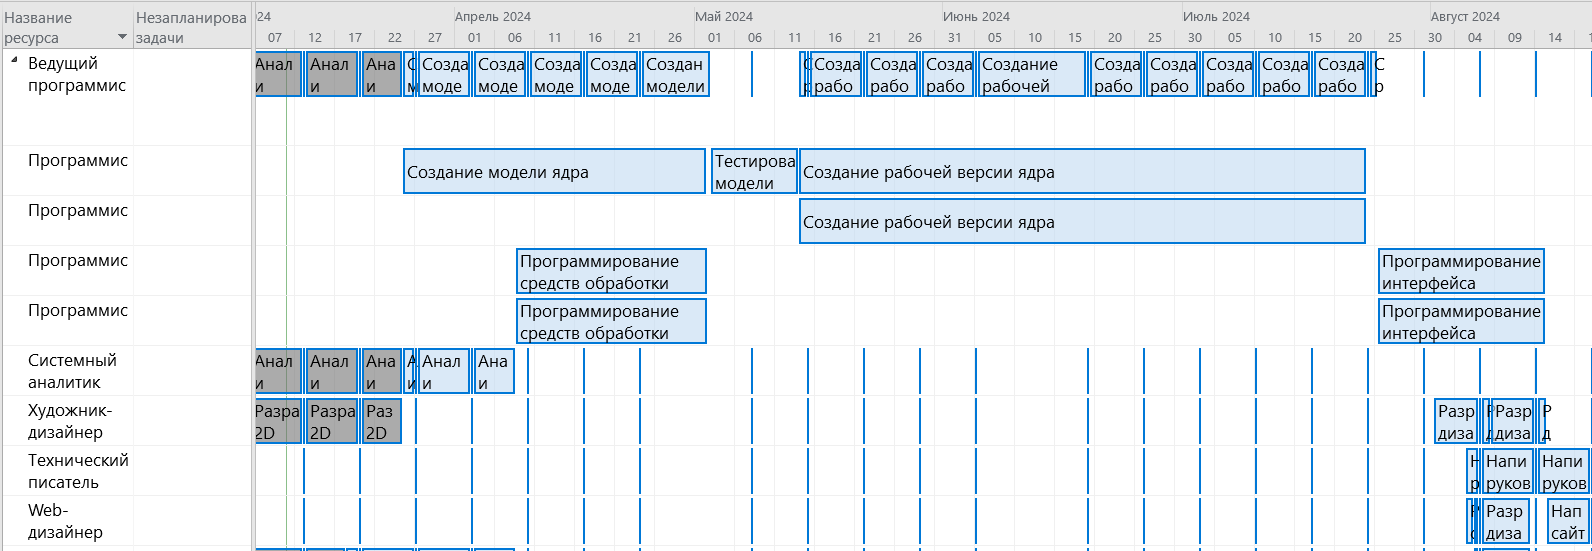
\includegraphics[scale=0.4]{inc/img/p_15.png}
	\end{center}
	\captionsetup{justification=centering}
	\label{fig:u3}
\end{figure}

Поскольку тип задачи по умолчанию – фиксированные трудозатраты, то
уменьшать время нужно за счет увеличения единиц ресурсов.

Оптимизируем участие программистов в этих задачах.

\begin{figure}[h!]
	\begin{center}
		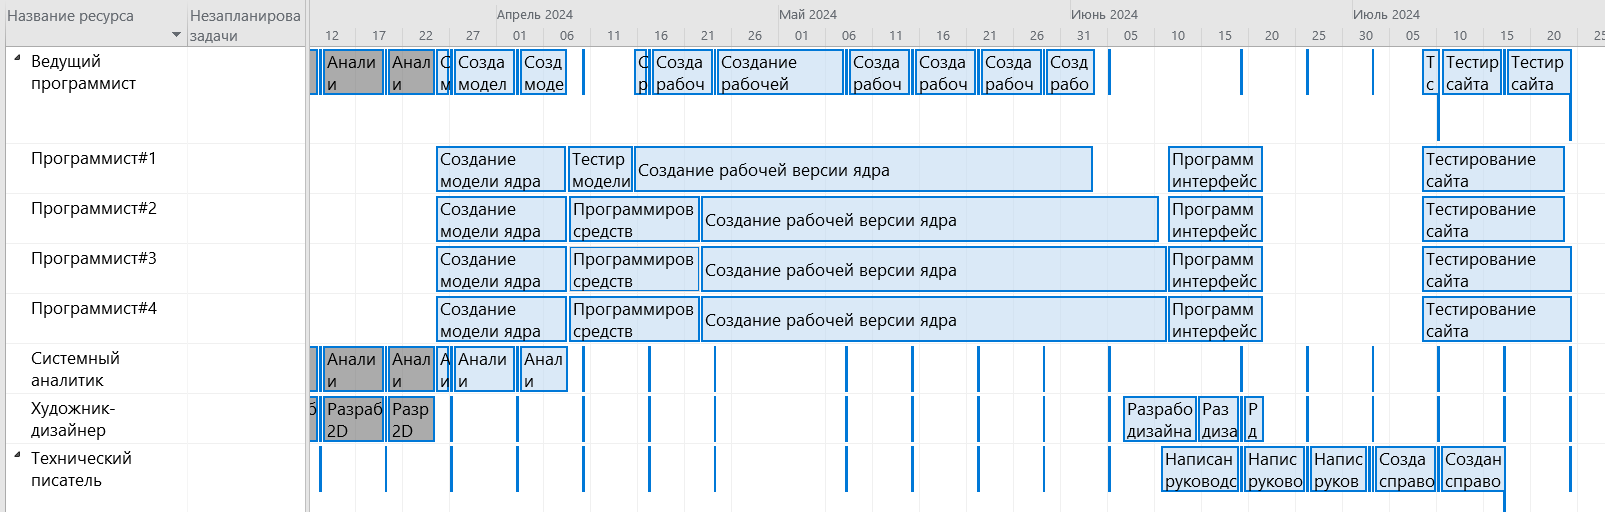
\includegraphics[scale=0.38]{inc/img/p_16.png}
	\end{center}
	\captionsetup{justification=centering}
	\label{fig:u3}
\end{figure}

\newpage

Получили следующие результаты.

\begin{figure}[h!]
	\begin{center}
		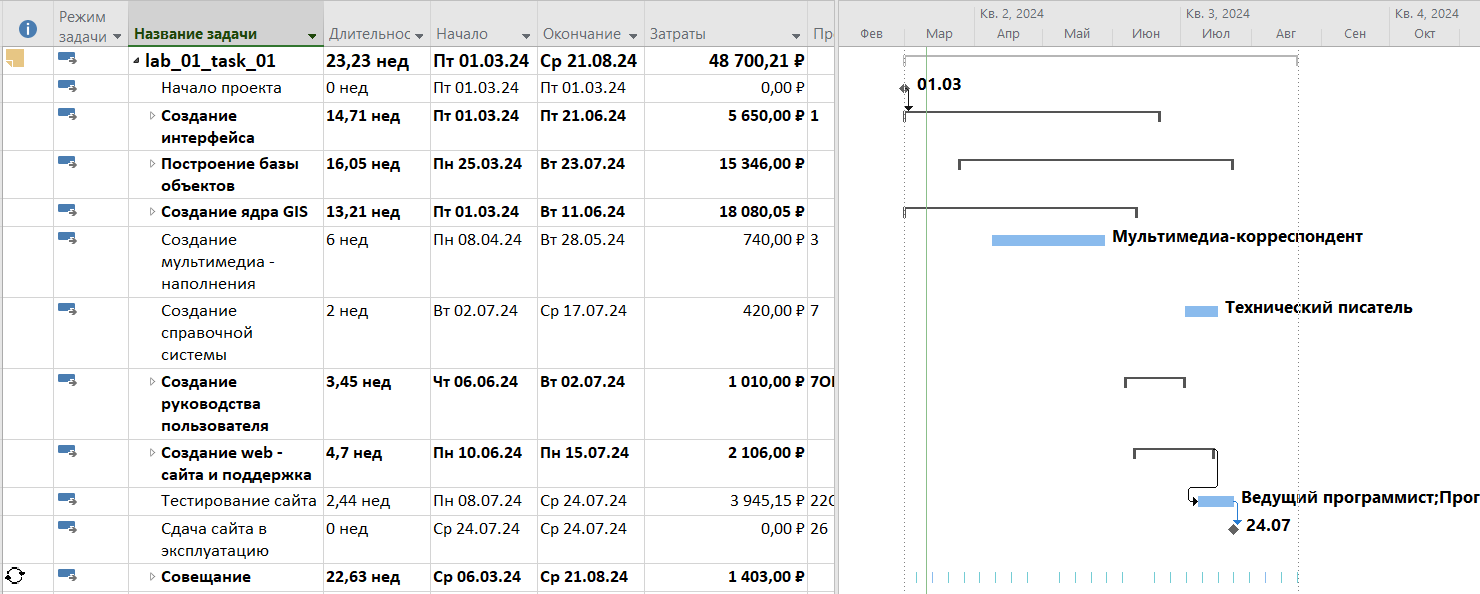
\includegraphics[scale=0.38]{inc/img/p_17.png}
	\end{center}
	\captionsetup{justification=centering}
	\label{fig:u3}
\end{figure}

Теперь удалим совещания, которые происходят после сдачи сайта в
эксплуатацию (кроме первого 24.07, на случай если что-то пойдет не так).

\begin{figure}[h!]
	\begin{center}
		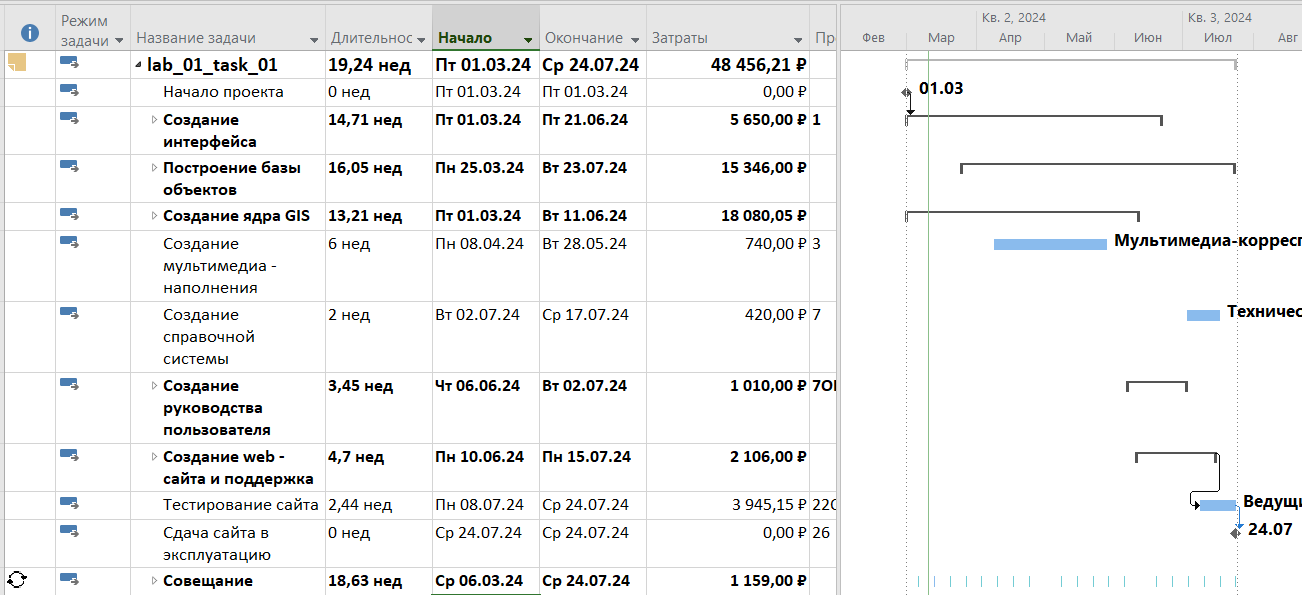
\includegraphics[scale=0.4]{inc/img/p_18.png}
	\end{center}
	\captionsetup{justification=centering}
	\label{fig:u3}
\end{figure}

Таким образом, удалось уменьшить срок исполнения проекта с 28,58 недель до 19,24 и затраты с 49825 до 48456. И то, и то укладывается в заданные рамки.

Проанализируем, как изменилось после оптимизации соотношение
«Трудозатраты – Затраты» по группам ресурсов, взяв за основу результаты выполнения Задания №3 Лабораторной работы №2. 

До оптимизации

\begin{figure}[h!]
	\begin{center}
		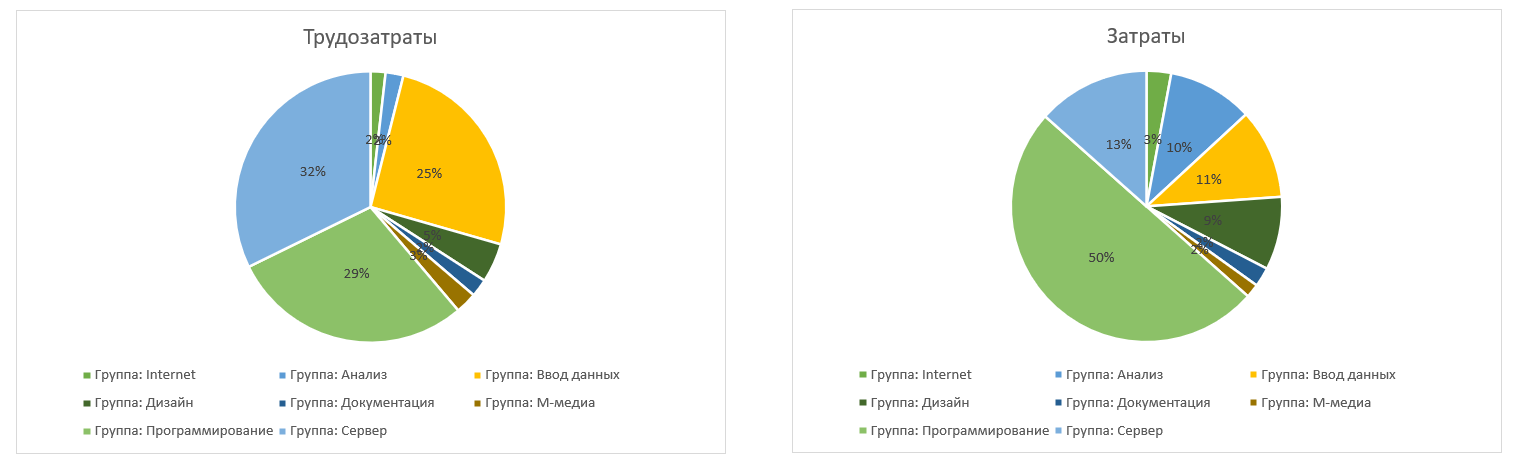
\includegraphics[scale=0.44]{inc/img/p_19.png}
	\end{center}
	\captionsetup{justification=centering}
	\label{fig:u3}
\end{figure}

После оптимизации 

\begin{figure}[h!]
	\begin{center}
		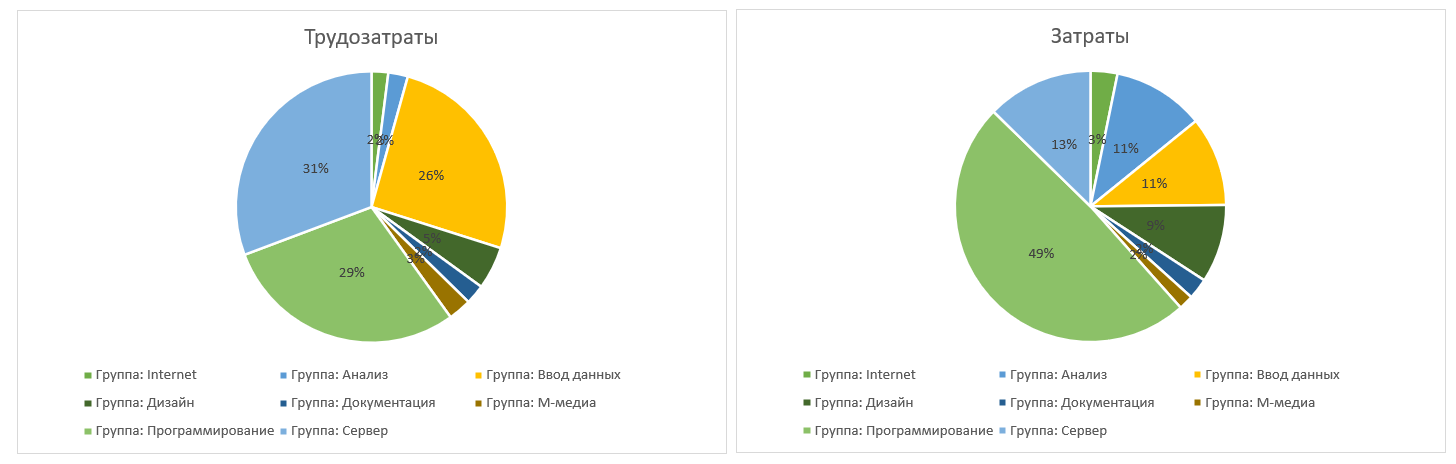
\includegraphics[scale=0.45]{inc/img/p_20.png}
	\end{center}
	\captionsetup{justification=centering}
	\label{fig:u3}
\end{figure}

Таким образом, соотношение трудозатрат к затратам практически не изменилось. 

Также был сохранен базовый план:

\begin{figure}[h!]
	\begin{center}
		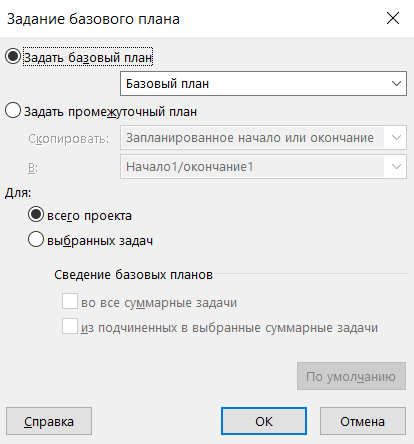
\includegraphics[scale=0.38]{inc/img/p_21.png}
	\end{center}
	\captionsetup{justification=centering}
	\label{fig:u3}
\end{figure}

\newpage

\subsection*{Вывод}

Таким образом, благодаря выравниванию загрузки ресурсов в проекте удалось избавиться от их перегрузки.

Были добавлены регулярные совещания, затраты на которые удалось
уменьшить за счет введения отдельных планов для участвующих в них сотрудниках.

При анализе критического пути в проекте и результатов оптимизатора ресурсов были выявлены задачи, которые сильнее всего влияли на увеличение сроков выполнения проекта. Этим задачам были добавлены дополнительные ресурсы (программисты), благодаря чему удалось сократить сроки выполнения данных задач, а, следовательно, и всего проекта в целом.

В итоге затраты составили 48 456 при ограничении в 50 000 (было
48 825), а сроки исполнения проекта – 19,24 недели при
ограничении в 6 месяцев (было 28,56 недель без учета совещаний), дата окончания проекта – 24.07.23.

При этом соотношение «Трудозатраты – Затраты» по группам ресурсов в результате выравнивания и переназначения ресурсов практически не изменилось.